\graphicspath{{./assets/}}
\setcounter{mtc}{6}
\chapter{4th Sprint : Preliminary infrastructure setup}
\fancyhead[R]{\ungaramond\small\textbf{Chapter VI.  4th Sprint: Preliminary infrastructure setup  }}

\minitoc
\newpage
\section*{Introduction}

\section{Sprint backlog :}

\begin{longtable}[H]{|m{1.5cm}|m{3cm}|m{1.5cm}|m{9cm}|}
\hline
{\textbf{Epic ID}} & {\textbf{Epic}} & {\textbf{Story ID}} & {\textbf{Story}}\\
\hline
1  & Setup and configuration of provisioned resources using ansible playbooks.	 &  1.1	 &  Writing resource-specific roles to setup the resources. \\
\cline{3-4}
& & 1.2 & Configuring the written roles into playbook. \\
\cline{3-4}
& & 1.3	& Starting the infrastructure setup process. \\
\cline{3-4}
\hline
\caption{4th Sprint Backlog}
\end{longtable}

\section{UML design: activity diagram for infrastructure setup}

This activity diagram illustrates how Ansible and Terraform can work together to provision infrastructure resources and set up a PaaS environment.

\begin{figure}[H]\centering
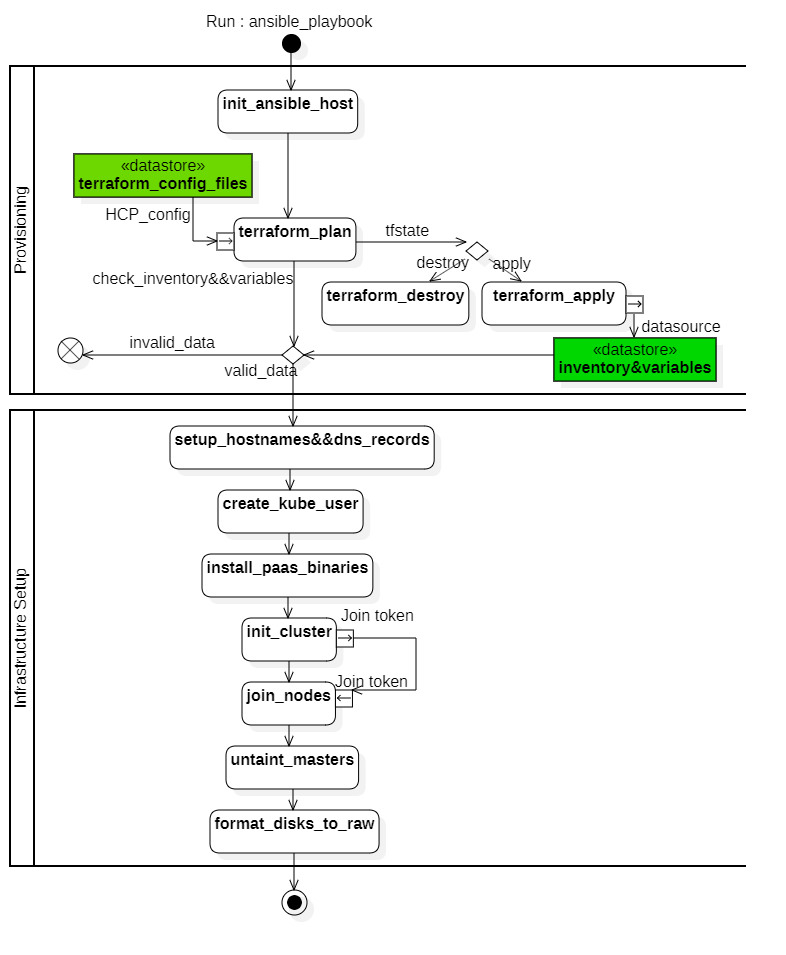
\includegraphics[width=1.0\textwidth,angle=00]{assets/f20.png}
\caption{Activity diagram for infrastructure setup}
\label{fig:activity diagram for infrastructure setup}
\end{figure}


\section{UML design: sequence diagram for infrastructure setup}

The following is a sequence diagram that shows the flow of actions or events that occur during the process of setting up the infrastructure.


\begin{figure}[H]\centering
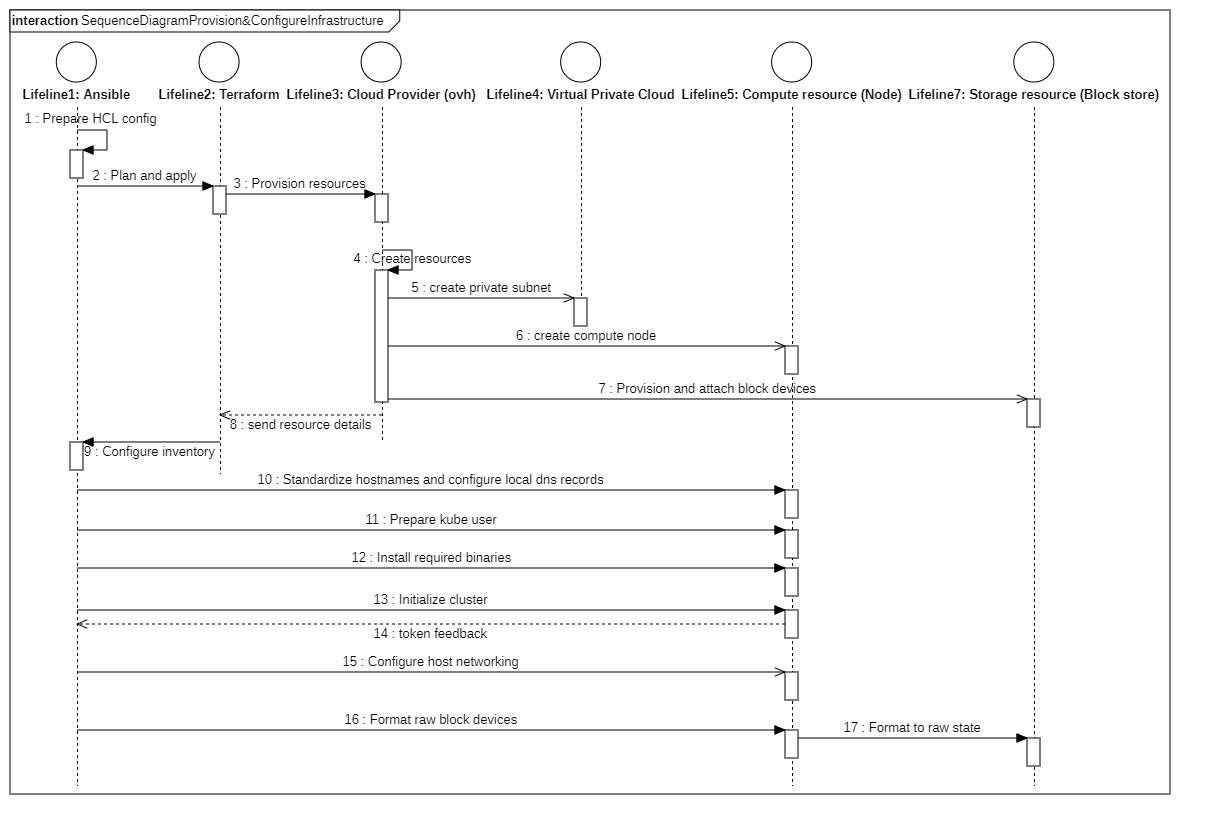
\includegraphics[width=1.0\textwidth,angle=00]{assets/f16.png}
\caption{Sequence diagram for infrastructure setup}
\label{fig:Sequence diagram for infrastructure setup}
\end{figure}

\begin{itemize}[label={--}]
    \item The user initiates the infrastructure setup process by running starting an ansible playbook.
    \item The first ansible playbook sets up the host machine to run terraform. It invokes Terraform, which then communicates with the OVH API to provision the required resources.
    \item OVH API receives the request and creates the necessary resources such as virtual machines, block storage volumes, and network interfaces.
    \item Terraform receives the response from the OVH API and applies any necessary configurations to the provisioned resources.
    \item Ansible then takes over and configures the provisioned resources by installing the required packages, setting up the network configurations, and configuring the software applications.
    \item If everything is working as expected, a notification is sent via an office 360 webhook channel. The devSecOps team is notified that the infrastructure setup process is complete, and the system is ready for use.
\end{itemize}

\section{Playbook diagrams for resource setup}

\subsection{Playbook 0: Setting up individual instances}

Next, we look at the playbook for setting up and standardizing the both the ansible host and the public cloud instances.

\begin{figure}[H]\centering
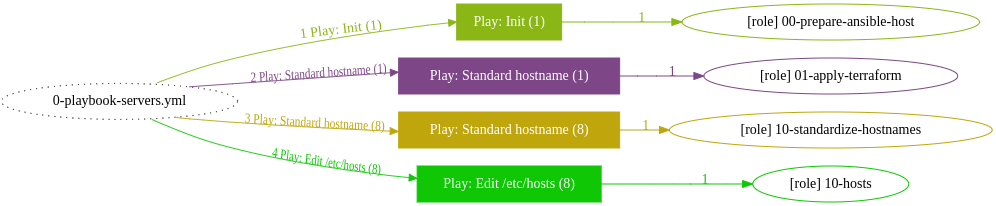
\includegraphics[width=1.0\textwidth,angle=00]{assets/f17.png}
\caption{individual instances diagram}
\label{fig:individual instances diagram}
\end{figure}

\subsection{Playbook 1: Orchestrated cluster setup}

For setting up the Kubernetes cluster on the provisioned infrastructure resources, the following step were automated using an ansible playbook:

\begin{itemize}[label={--}]
    \item The playbook first sets up the necessary prerequisites on each node, such as disabling swap, disabling firewall, installing necessary packages, etc.
    \item Next, it initializes the first node from the control plane as a master and joins the others as secondary masters. This involves setting up the necessary configuration files, certificates, and keys for the Kubernetes control plane.
    \item After the master node is initialized, the playbook joins the worker nodes. This involves passing the appropriate configuration information, such as the API server address and token, to the worker nodes.
    \item Once all nodes are part of the cluster, the playbook sets up networking using the CNI plugin Calico. This involves deploying the necessary network configuration files and pods to allow communication between nodes.
    \item Finally, the playbook sets up any necessary add-ons or customizations to the cluster, such as untainting master nodes, formatting block volumes to raw, adding custom scripts to switch between namespaces and contexts easily.
\end{itemize}

\begin{figure}[H]\centering
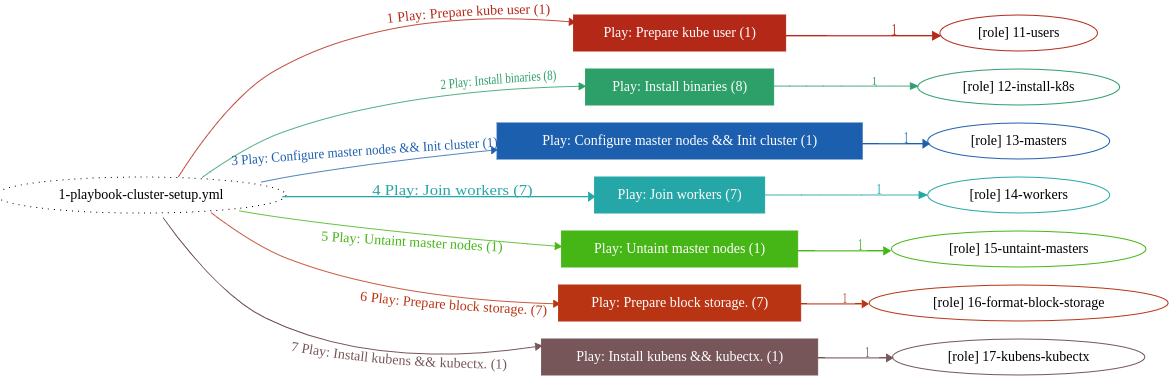
\includegraphics[width=1.0\textwidth,angle=00]{assets/f18.png}
\caption{Orchestrated cluster Diagram}
\label{fig:fig18}
\end{figure}

A summary of the previous two diagrams is depicted in the following figure :

\begin{figure}[H]\centering
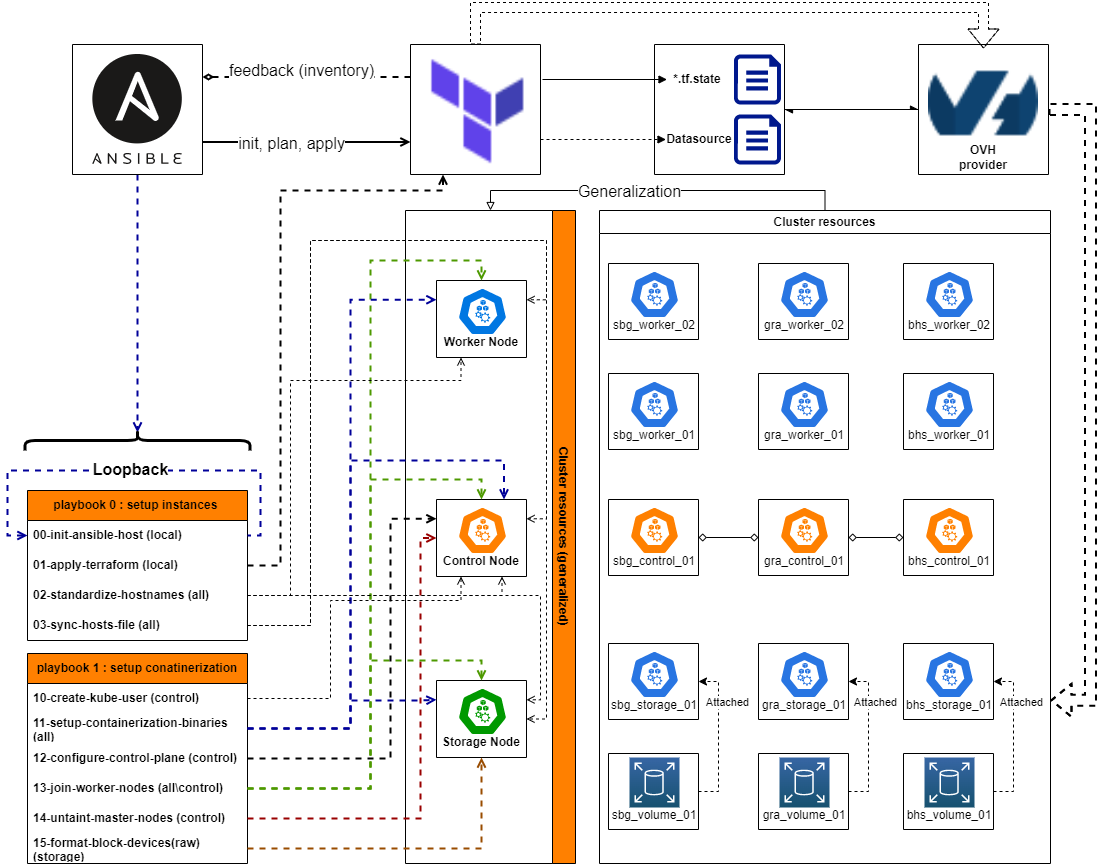
\includegraphics[width=1.0\textwidth,angle=00]{assets/f19.png}
\caption{Orchestrated cluster setup}
\label{fig:Orchestrated cluster setup}
\end{figure}

\section*{Conclusion}


Overall, the playbook aims to automate the setup and configuration of the Kubernetes to prepare it to host the various PaaS services that will be seen next chapter, allowing for consistent and repeatable deployments of Kubernetes infrastructure.

